%% USPSC-RELAT-modelo.tex
% ---------------------------------------------------------------
% USPSC: Modelo de Trabalho Academico (tese de doutorado, dissertacao de
% mestrado e trabalhos monograficos em geral) em conformidade com 
% ABNT NBR 14724:2011: Informacao e documentacao - Trabalhos academicos -
% Apresentacao
%----------------------------------------------------------------
%% Esta é uma customização do abntex2-modelo-trabalho-academico.tex de v-1.9.5 laurocesar 
%% para as Unidades do Campus USP de São Carlos:
%% EESC - Escola de Engenharia de São Carlos
%% IAU - Instituto de Arquitetura e Urbanismo
%% ICMC - Instituto de Ciências Matemáticas e de Computação
%% IFSC - Instituto de Física de São Carlos
%% IQSC - Instituto de Química de São Carlos
%%
%% Este trabalho utiliza a classe USPSC.cls que é mantida pela seguinte equipe:
%% 
%% Coordenação e Programação:
%%   - Marilza Aparecida Rodrigues Tognetti - marilza@sc.usp.br (PUSP-SC)
%%   - Ana Paula Aparecida Calabrez - aninha@sc.usp.br (PUSP-SC)
%% Normalização:
%%   - Brianda de Oliveira Ordonho Sigolo - brianda@usp.br (IAU)
%%   - Eduardo Graziosi Silva - edu.gs@sc.usp.br (EESC)
%%   - Eliana de Cássia Aquareli Cordeiro - eliana@iqsc.usp.br (IQSC)
%%   - Flávia Helena Cassin - cassinp@sc.usp.br (EESC)
%%   - Maria Cristina Cavarette Dziabas - mcdziaba@ifsc.usp.br (IFSC)
%%   - Regina Célia Vidal Medeiros - rcvmat@icmc.usp.br (ICMC)
%%
%% O USPSC-modelo.tex e USPSC-TCC-modelo.tex utilizam diversos arquivos relacionado em 
%% 2.1 Pacote USPSC: Classe USPSC e modelos de trabalhos acadêmicos	do Tutorial do Pascote 
%%  USPSC para modelos de trabalhos de acadêmicos em LaTeX - versão 3.1


%----------------------------------------------------------------
%% Sobre a classe abntex2.cls:
%% abntex2.cls, v-1.9.5 laurocesar
%% Copyright 2012-2015 by abnTeX2 group at https://www.abntex.net.br/ 
%%
%----------------------------------------------------------------
%\documentclass[french,12pt,openany,oneside,openright]{memoir}

\documentclass[
% -- opções da classe memoir --
openany % Capítulos na mesma página
12pt,		% tamanho da fonte
openright,	% capítulos começam em pág ímpar (insere página vazia caso preciso)
%twoside,  % para impressão em anverso (frente) e verso. Oposto a oneside - Nota: utilizar \imprimirfolhaderosto*
oneside, % para impressão em páginas separadas (somente anverso) -  Nota: utilizar \imprimirfolhaderosto
% inclua uma % antes do comando twoside e exclua a % antes do oneside 
a4paper,			% tamanho do papel. 
% -- opções da classe abntex2 --
chapter=TITLE,		% títulos de capítulos convertidos em letras maiúsculas
% -- opções do pacote babel --
english,			% idioma adicional para hifenização
french,				% idioma adicional para hifenização
spanish,			% idioma adicional para hifenização
brazil				% o último idioma é o principal do documento
% {USPSC-classe/USPSC} configura o cabeçalho contendo apenas o número da página
]{USPSC-classe/USPSC}
%]{USPSC-classe/USPSC1}
% Inclua % antes de ]{USPSC-classe/USPSC} e retire a % antes de %]{USPSC-classe/USPSC1} para utilizar o 
% cabeçalho diferenciado para as páginas pares e ímpares:
%- páginas ímpares: com seções ou subseções e o número da página
%- páginas pares: com o número da página e o título do capítulo 
% ---
% ---
% Pacotes básicos - Fundamentais 
% ---
\usepackage[T1]{fontenc}		% Seleção de códigos de fonte.
\usepackage[utf8]{inputenc}		% Codificação do documento (conversão automática dos acentos)
\usepackage{lmodern}			% Usa a fonte Latin Modern
% Para utilizar a fonte Times New Roman, inclua uma % no início do comando acima  "\usepackage{lmodern}"
% Abaixo, tire a % antes do comando  \usepackage{times}
%\usepackage{times}		    	% Usa a fonte Times New Roman	
% Para usar a fonte , lembre-se de tirar a % do comando %\renewcommand{\ABNTEXchapterfont}{\rmfamily}, localizado mais abaixo, logo após "Outras opções para nota de rodapé no Sistema Numérico" 					
\usepackage{lastpage}			% Usado pela Ficha catalográfica
\usepackage{indentfirst}		% Indenta o primeiro parágrafo de cada seção.
\usepackage{color}				% Controle das cores
\usepackage{graphicx}			% Inclusão de gráficos
\usepackage{float} 				% Fixa tabelas e figuras no local exato
\usepackage{chemfig}            % Para escrever reações químicas
\usepackage{chemmacros}         % Para escrever reações químicas
\usepackage{tikz}				% Para escrever reações químicas e outros
\usetikzlibrary{positioning}
\usepackage{microtype} 			% para melhorias de justificação
\usepackage{pdfpages}
\usepackage{makeidx}            % para gerar índice remissivo
\usepackage{hyphenat}          % Pacote para retirar a hifenizacao do texto
\usepackage[absolute]{textpos} % Pacote permite o posicionamento do texto
\usepackage{eso-pic}           % Pacote para incluir imagem de fundo
\usepackage{makebox}           % Pacote para criar caixa de texto
% ---

% ---
% Pacotes de citações
% Citações padrão ABNT
% ---
% Sistemas de chamada: autor-data ou numérico.
% Sistema autor-data
\usepackage[alf, abnt-emphasize=bf, abnt-thesis-year=both, abnt-repeated-author-omit=no, abnt-last-names=abnt, abnt-etal-cite=3, abnt-etal-list=3, abnt-etal-text=it, abnt-and-type=e, abnt-doi=doi, abnt-url-package=none, abnt-verbatim-entry=no]{abntex2cite}
\bibliographystyle{USPSC-classe/abntex2-alf-USPSC}
% Se o idioma for o inglês, inclua % no comando acima e exclua o % do comando abaixo
%\bibliographystyle{USPSC-classe/abntex2-alfeng-USPSC}

% Para o IQSC, que indica todos os autores nas referências, incluir % no início dos comandos acima e retirar a % dos comandos abaixo 
%\usepackage[alf, abnt-emphasize=bf, abnt-thesis-year=both, abnt-repeated-author-omit=no, abnt-last-names=abnt, abnt-etal-cite=3, abnt-etal-list=0, abnt-etal-text=it, abnt-and-type=e, abnt-doi=doi, abnt-url-package=none, abnt-verbatim-entry=no]{abntex2cite} 
%\bibliographystyle{USPSC-classe/abntex2-alf-USPSC}
% Se o idioma for o inglês, exclua % no comando acima ou do comando abaixo
%\bibliographystyle{USPSC-classe/abntex2-alfeng-USPSC}

% Sistema Numérico
% Para citações numéricas, sistema adotado pelo IFSC, incluir % no início dos comandos acima e retirar a % dos comandos abaixo 
%\usepackage{cite}              % agrupa citações numéricas consecutivas
%\usepackage[num, abnt-emphasize=bf, abnt-thesis-year=both, abnt-repeated-author-omit=no, abnt-last-names=abnt, abnt-etal-cite=3, abnt-etal-list=3, abnt-etal-text=it, abnt-and-type=e, abnt-doi=doi, abnt-url-package=none, abnt-verbatim-entry=no]{abntex2cite} 
%\bibliographystyle{USPSC-classe/abntex2-num-USPSC}
% Se o idioma for o inglês, exclua % no comando acima ou do comando abaixo
%\bibliographystyle{USPSC-classe/abntex2-numeng-USPSC}

% Complementarmente, verifique as instruções abaixo sobre os Pacotes de Nota de rodapé
% ---
% Pacotes de Nota de rodapé
% Configurações de nota de rodapé

% O presente modelo adota o formato numérico para as notas de rodapés quando utiliza o sistema de chamada autor-data para citações e referências. Para utilizar o sistema de chamada numérico para citações e referências, habilitar um dos comandos abaixo.
% Há diversa opções para nota de rodapé no Sistema Numérico.  Para o IFSC, habilitade o comando abaixo.

%\renewcommand{\thefootnote}{\fnsymbol{footnote}}  %Comando para inserção de símbolos em nota de rodapé

% Outras opções para nota de rodapé no Sistema Numérico:
%\renewcommand{\thefootnote}{\alph{footnote}}      %Comando para inserção de letras minúscula em nota de rodapé
%\renewcommand{\thefootnote}{\Alph{footnote}}      %Comando para inserção de letras maiúscula em nota de rodapé
%\renewcommand{\thefootnote}{\roman{footnote}}     %Comando para inserção de números romanos minúsculos  em nota de rodapé
%\renewcommand{\thefootnote}{\Roman{footnote}}     %Comando para inserção de números romanos minúsculos  em nota de rodapé

\renewcommand{\footnotesize}{\small} %Comando para diminuir a fonte das notas de rodapé
%Para utilizar a fonte Times New Roman, inclua retire % do início do comando abaixo 
%\renewcommand{\ABNTEXchapterfont}{\rmfamily}

% ---
% Pacote para agrupar a citação numérica consecutiva
% Quando for adotado o Sistema Numérico, a exemplo do IFSC, habilite 
% o pacote cite abaixo retirando a porcentagem antes do comando abaixo
%\usepackage[superscript]{cite}	

% ---
% Pacotes adicionais, usados apenas no âmbito do Modelo Canônico do abnteX2
% ---
\usepackage{lipsum}				% para geração de dummy text
% ---

% pacotes de tabelas
\usepackage{multicol}	% Suporte a mesclagens em colunas
\usepackage{multirow}	% Suporte a mesclagens em linhas
\usepackage{longtable}	% Tabelas com várias páginas
\usepackage{threeparttablex}    % notas no longtable
\usepackage{array}

% ----
% Compatibilização com a ABNT NBR 6023:2018 e 10520:2023
% Para tirar <> da URL e tornar as expressões latinas em itálico
\usepackage{USPSC-classe/ABNT6023-10520}
% As demais compatibilizações estão nos arquivos abntex2-alf-USPSC.bst,abntex2-alfeng-USPSC.bst, abntex2-num-USPSC.bst e abntex2-numeng-USPSC.bst, dependendo do idioma do textos e se o sistemas de chamada for autor-data ou numérico, conforme explicitado acima.
% ----

% ---
% DADOS INICIAIS - Define sigla com título, área de concentração e opção do Programa 
% Consulte a tabela referente aos Programas, áreas e opções de sua unidade contante do
% arquivo USPSC-Siglas estabelecidas para os Programas de Pós-Graduação por Unidade.xlsx 
% ou nos APÊNDICES A-F
\siglaunidade{OUTROS-RELAT}
\programa{XXXX}
% Os demais dados deverão ser fornecidos no arquivo USPSC-pre-textual-UUUU ou USPSC-TCC-pre-textual-UUUU, onde UUUU é a sigla da Unidade. 
% Exemplo:USPSC-pre-textual-IFSC.tex
% ---
% Configurações de aparência do PDF final
% alterando o aspecto da cor azul
\definecolor{blue}{RGB}{41,5,195}

% informações do PDF
\makeatletter
\hypersetup{
	%pagebackref=true,
	pdftitle={\@title}, 
	pdfauthor={\@author},
	pdfsubject={\imprimirpreambulo},
	pdfcreator={LaTeX with abnTeX2},
	pdfkeywords={abnt}{latex}{abntex}{USPSC}{trabalho acadêmico}, 
	colorlinks=true,       		% false: boxed links; true: colored links
	linkcolor=black,          	% color of internal links
	citecolor=black,        		% color of links to bibliography
	filecolor=black,      		% color of file links
	urlcolor=black,
	%Para habilitar as cores dos links, retire a % antes dos comandos abaixo e inclua a % antes das 4 linhas de comando acima 
	%linkcolor=blue,            	% color of internal links
	%citecolor=blue,        		% color of links to bibliography
	%filecolor=magenta,      		% color of file links
	%urlcolor=blue,
	bookmarksdepth=4	
}
\makeatother
% --- 
% ----
% Início do documento
% ----
\begin{document}

% Seleciona o idioma do documento (conforme pacotes do babel)
\selectlanguage{brazil}
% Se o idioma do texto for inglês, inclua uma % antes do 
%      comando \selectlanguage{brazil} e 
%      retire a % antes do comando abaixo
%\selectlanguage{english}

% Retira espaço extra obsoleto entre as frases.
\frenchspacing 

% --- Formatação dos Títulos
\renewcommand{\ABNTEXchapterfontsize}{\fontsize{12}{12}\bfseries}
\renewcommand{\ABNTEXsectionfontsize}{\fontsize{12}{12}\bfseries}
\renewcommand{\ABNTEXsubsectionfontsize}{\fontsize{12}{12}\normalfont}
\renewcommand{\ABNTEXsubsubsectionfontsize}{\fontsize{12}{12}\normalfont}
\renewcommand{\ABNTEXsubsubsubsectionfontsize}{\fontsize{12}{12}\normalfont}

% ----------------------------------------------------------
% ELEMENTOS PRÉ-TEXTUAIS
% ----------------------------------------------------------
% ---
% Folha de rosto do relatório
% (o * indica impressão em anverso (frente) e verso )
% ---
\imprimirfolhaderostoalt*
%\imprimirfolhaderostoalt

% ---
% ---
% Inserir informações no verso da página 
% Indicar a equipe técnica, elemento opcional, indica a comissão de estudo, colaboradores, coordenação geral entre outros.
%NOTA Pode ser incluída na folha subsequente à folha de rosto, a ficha catalográfica em pdf
% ---
% Altere o arquivo USPSC-VersoPaginaDeRosto-Relatorio.doc com as informações da equipe
% e salve-o como PDF na pasta USPSC-TA-PreTextual 
% e inclua o arquivo utilizando o comando abaixo:

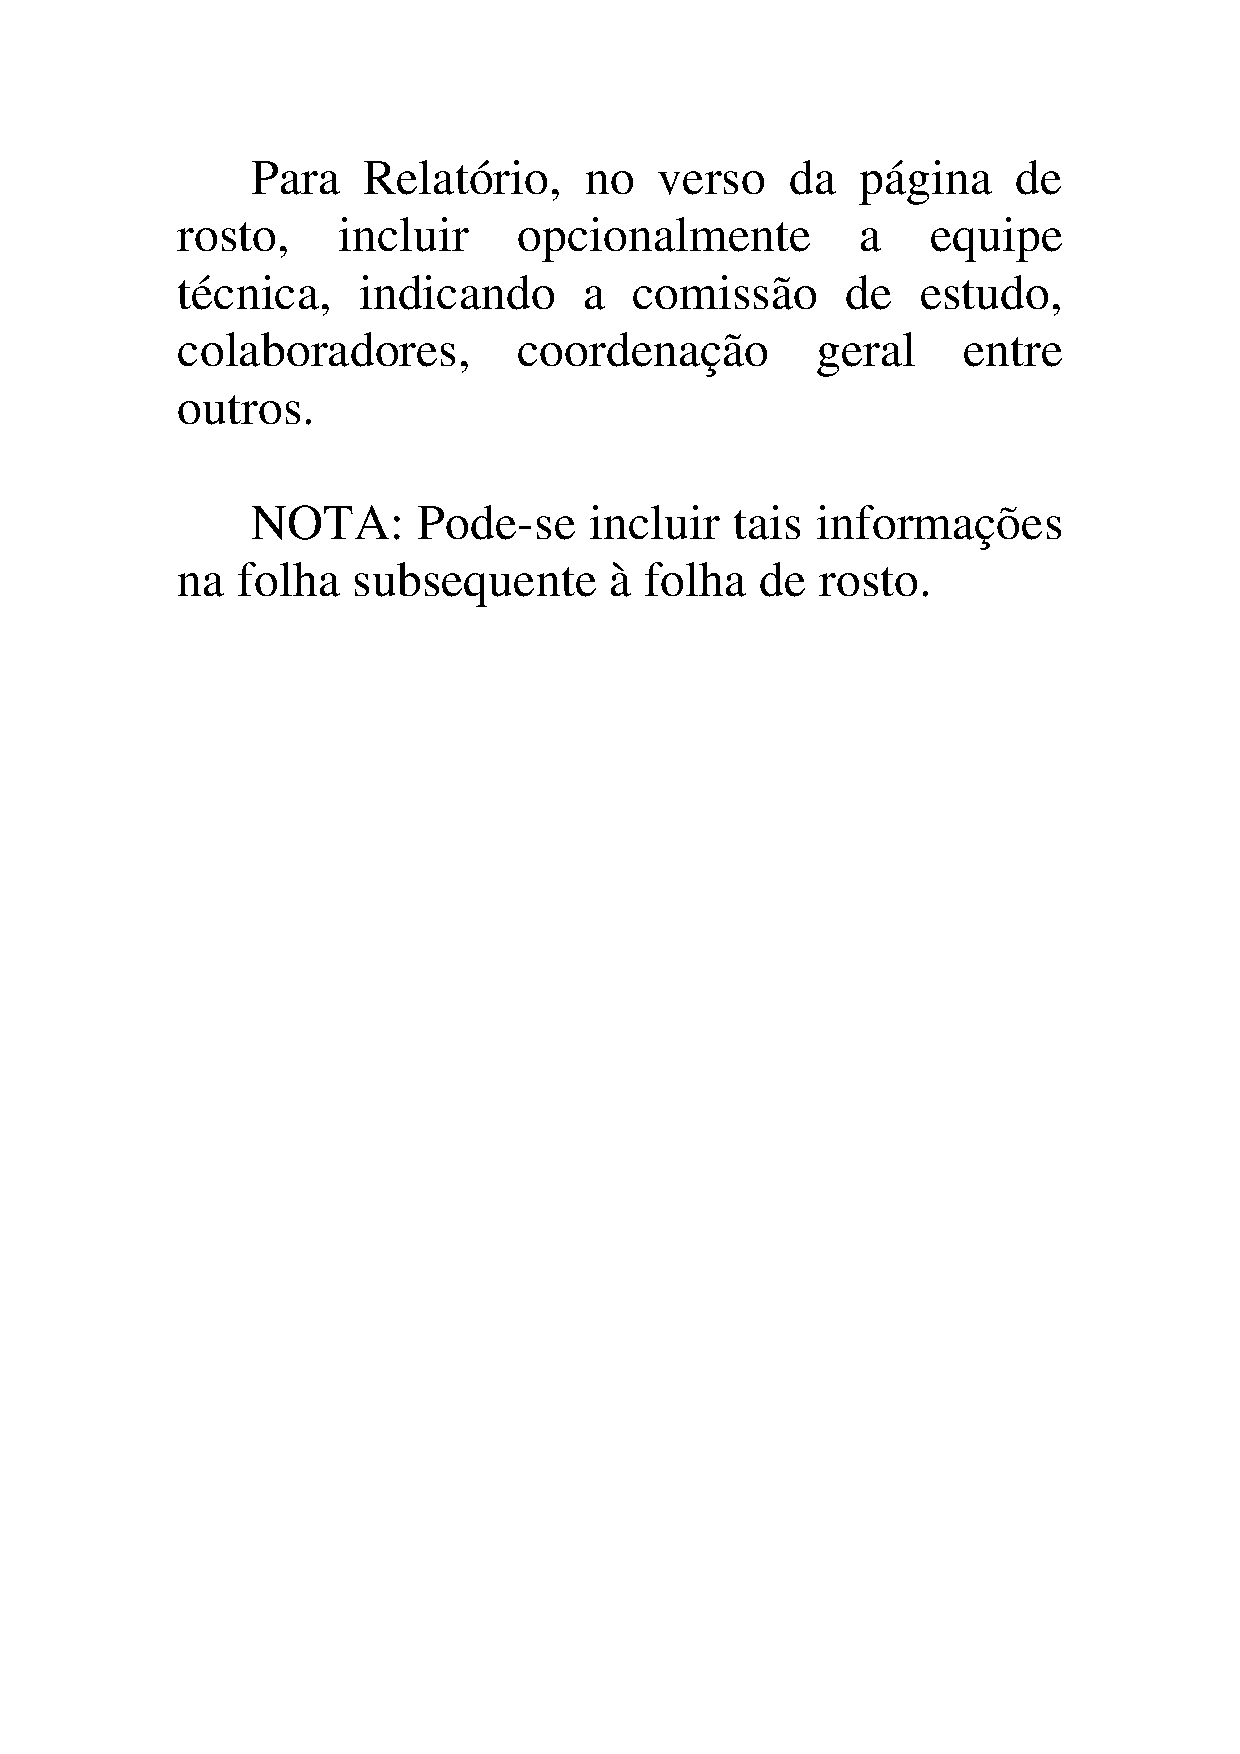
\includepdf{USPSC-TA-PreTextual/USPSC-VersoPaginaDeRosto-Relatorio.pdf}

% ---
% Resumo
% ---
%% USPSC-Resumo.tex
\setlength{\absparsep}{18pt} % ajusta o espaçamento dos parágrafos do resumo		
\begin{resumo}
	\begin{flushleft} 
			\setlength{\absparsep}{0pt} % ajusta o espaçamento da referência	
			\SingleSpacing 
			\imprimirautorabr~~\textbf{\imprimirtituloresumo}.	\imprimirdata. \pageref{LastPage} p. 
			%Substitua p. por f. quando utilizar oneside em \documentclass
			%\pageref{LastPage} f.
			\imprimirtipotrabalho~-~\imprimirinstituicao, \imprimirlocal, \imprimirdata. 
 	\end{flushleft}
\OnehalfSpacing 			
 O resumo deve ressaltar o  objetivo, o método, os resultados e as conclusões do documento. A ordem e a extensão  destes itens dependem do tipo de resumo (informativo ou indicativo) e do  tratamento que cada item recebe no documento original. O resumo deve ser
 precedido da referência do documento, com exceção do resumo inserido no
 próprio documento. (\ldots)  Salientamos que algumas Unidades exigem o titulo dos trabalhos acadêmicos em inglês, tornando necessário a inclusão das referências nos resumos e abstracts, o que foi adotado no \textbf{Modelo para TCC em \LaTeX\ utilizando a classe USPSC} e no \textbf{Modelo para teses e dissertações em \LaTeX\ utilizando a classe USPSC}. As palavras-chave devem figurar logo abaixo do  resumo, antecedidas da expressão Palavras-chave:, separadas entre si por  ponto e finalizadas também por ponto \cite{nbr6028}.
 

 \textbf{Palavras-chave}: LaTeX. Classe USPSC. Tese. Dissertação. Trabalho de conclusão de curso (TCC). Relatório.
\end{resumo}
% ---
%página em branco

\includepdf{USPSC-TA-PreTextual/USPSC-PaginaEmBranco.pdf}
% ----------------------------------------------------------
% ELEMENTOS TEXTUAIS
% ----------------------------------------------------------
\textual
% Os capítulos são inseridos como arquivos externos
%% Enibir mudança de páginas entre capítulos
\begingroup
\renewcommand{\cleardoublepage}{}
\renewcommand{\clearpage}{}
\setlength\afterchapskip{\lineskip} 
% ---
% Capítulo 1 - Introdução
% ---
%% USPSC-Introducao.tex

% ----------------------------------------------------------
% Introdução (exemplo de capítulo sem numeração, mas presente no Sumário)
% ----------------------------------------------------------
\chapter[Introdução]{Introdução}
\label{Introdução}


Parte inicial do texto, que contém a delimitação do assunto tratado, objetivos da pesquisa e outros elementos necessários para apresentar o tema do trabalho \cite{aguia2020}.

% ---
\vspace{1.0cm}

% ---
% Capítulo 2
% ---
%% USPSC-Cap2-Desenvolvimento.tex 

% ---
% Este capítulo, utilizado por diferentes exemplos do abnTeX2, ilustra o uso de
% comandos do abnTeX2 e de LaTeX.
% ---

\chapter{Desenvolvimento}\label{cap_exemplos}
Este capítulo é parte principal do trabalho acadêmico e deve conter a exposição ordenada e detalhada do assunto. Divide-se em seções e subseções, em conformidade com a abordagem do tema e do método, abrangendo: revisão bibliográfica, materiais e métodos, técnicas utilizadas, resultados obtidos e discussão.

Abaixo são apresentados minimamente exemplos tabelas, quadros, divisões de documentos e outros itens. Consulte o \textbf{Tutorial do Pacote USPSC para modelos de trabalhos de acad\^emicos em LaTeX - vers\~ao 3.2} para demais informações. 

\section{Resultados de comandos}\label{sec-divisoes}

% ---
\subsection{Tabelas e quadros}

O \textbf{Tutorial do Pacote USPSC para modelos de trabalhos de acad\^emicos em LaTeX - vers\~ao 3.2} apresenta orientações completas e diversas formatações de tabelas, dentre elas a \autoref{tab-ibge}, que é um exemplo de tabela alinhada que pode ser longa ou curta, conforme padrão do Instituto Brasileiro de Geografia e Estatística (IBGE).

%\begin{table}[H]
\begin{table}[htb]
	\IBGEtab{%
		\caption{Frequência anual por categoria de usuários}%
		\label{tab-ibge}
	}{%
		\begin{tabular}{ccc}
			\toprule
			Categoria de Usuários & Frequência de Usuários \\
			\midrule \midrule
			Graduação & 72\% \\
			\midrule 
			Pós-Graduação & 15\% \\
			\midrule 
			Docente & 10\% \\
			\midrule 
			Outras & 3\% \\
			\bottomrule
		\end{tabular}%
	}{%
		\fonte{Elaborada pelos autores.}%
		\nota{Exemplo de uma nota.}%
		\nota[Anotações]{Uma anotação adicional, que pode ser seguida de várias
			outras.}%
		
	}
\end{table}

A formatação do quadro é similar à tabela, mas deve ter suas laterais fechadas e conter as linhas horizontais.

% o comando \newpage foi utilizado para forçar a quebra de página
%\newpage
\begin{quadro}[htb]
	\caption{\label{quadro_modelo}Níveis de investigação}
	\begin{tabular}{|p{2.6cm}|p{6.0cm}|p{2.25cm}|p{3.40cm}|}
		\hline
		\textbf{Nível de Investigação} & \textbf{Insumos}  & \textbf{Sistemas de Investigação}  & \textbf{Produtos}  \\
		\hline
		Meta-nível & Filosofia\index{filosofia} da Ciência  & Epistemologia &
		Paradigma  \\
		\hline
		Nível do objeto & Paradigmas do metanível e evidências do nível inferior &
		Ciência  & Teorias e modelos \\
		\hline
		Nível inferior & Modelos e métodos do nível do objeto e problemas do nível inferior & Prática & Solução de problemas \\ 
		\hline
	\end{tabular}
	\begin{flushleft}
		%\fonte{\citeonline{van1986}}
		Fonte: \citeonline{van1986}
	\end{flushleft}
\end{quadro} 


No \textbf{Tutorial do Pacote USPSC para modelos de trabalhos de acad\^emicos em LaTeX - vers\~ao 3.2} são apresentados mais exemplos de quadros.

% ---
\subsection{Figuras}\label{sec_figuras}
% ---
\index{figuras}Figuras podem ser criadas diretamente em \LaTeX,
como o exemplo da abaixo.

\begin{figure}[htb]
	\caption{\label{fig_circulo}A delimitação do espaço}
	\begin{center}
		\setlength{\unitlength}{5cm}
		\begin{picture}(1,1)
		\put(0,0){\line(0,1){1}}
		\put(0,0){\line(1,0){1}}
		\put(0,0){\line(1,1){1}}
		\put(0,0){\line(1,2){.5}}
		\put(0,0){\line(1,3){.3333}}
		\put(0,0){\line(1,4){.25}}
		\put(0,0){\line(1,5){.2}}
		\put(0,0){\line(1,6){.1667}}
		\put(0,0){\line(2,1){1}}
		\put(0,0){\line(2,3){.6667}}
		\put(0,0){\line(2,5){.4}}
		\put(0,0){\line(3,1){1}}
		\put(0,0){\line(3,2){1}}
		\put(0,0){\line(3,4){.75}}
		\put(0,0){\line(3,5){.6}}
		\put(0,0){\line(4,1){1}}
		\put(0,0){\line(4,3){1}}
		\put(0,0){\line(4,5){.8}}
		\put(0,0){\line(5,1){1}}
		\put(0,0){\line(5,2){1}}
		\put(0,0){\line(5,3){1}}
		\put(0,0){\line(5,4){1}}
		\put(0,0){\line(5,6){.8333}}
		\put(0,0){\line(6,1){1}}
		\put(0,0){\line(6,5){1}}
		\end{picture}
	\end{center}
	\legend{Fonte: \citeonline{equipeabntex2}}
\end{figure}

Consulte o \textbf{Tutorial do Pacote USPSC para modelos de trabalhos de acad\^emicos em LaTeX - vers\~ao 3.2} para conhecer mais recursos referentes à figuras. 


% ---
\vspace{1.0cm}

% ---
% Capítulo 3 - Considerações Finais
% ---
%% USPSC-RELAT-Cap3-ConsideracoesFinais.tex
% ---
% Considerações finais
% ---
\chapter{Considerações finais}
% ---
% O comando abaixo insere parágrafos aleatórios só para exemplificar
Apresentar as considerações finais do relatório técnico e/ou científico correspondentes à pesquisa ou estudo realizado.

% ---
\vspace{1.0cm}
% Controle do espaçamento entre um parágrafo e outro:
\setlength{\parskip}{1.0cm} 
% ----------------------------------------------------------
% ELEMENTOS PÓS-TEXTUAIS
% ----------------------------------------------------------
\postextual

% ----------------------------------------------------------

% -----------------------------------------------------------
% Referências bibliográficas
% ----------------------------------------------------------
\bibliography{USPSC-bib/USPSC-modelo-references}
% ----------------------------------------------------------
\endgroup
\end{document}
